%-------------------------------------------------------------------------------
\section{Influence of waves on sediment transport processes}
\label{chap:infl_waves}
%-------------------------------------------------------------------------------
In coastal zones, the effect of waves superimposed to a mean current (wave-induced or tidal) can have an impact on the behaviour of the seabed. Due to the reduced thickness of the bed boundary layer, the bottom shear stress increases largely and the resulting sand transport rate could be in many cases of one order of magnitude than in the case of currents alone.

\begin{figure}[H]%
  \begin{center}
\begin{tabular}{c}
\includegraphics[angle=180,origin=c,scale=0.15]{./graphics/fig_sed_waves.png}
\end{tabular}
\end{center}
\end{figure}

Underneath the wave surface, there is a fluid motion associated with the motion of the water surface, where the fluid particles describe an orbital path.

\begin{figure}[H]%
  \begin{center}
\begin{tabular}{c}
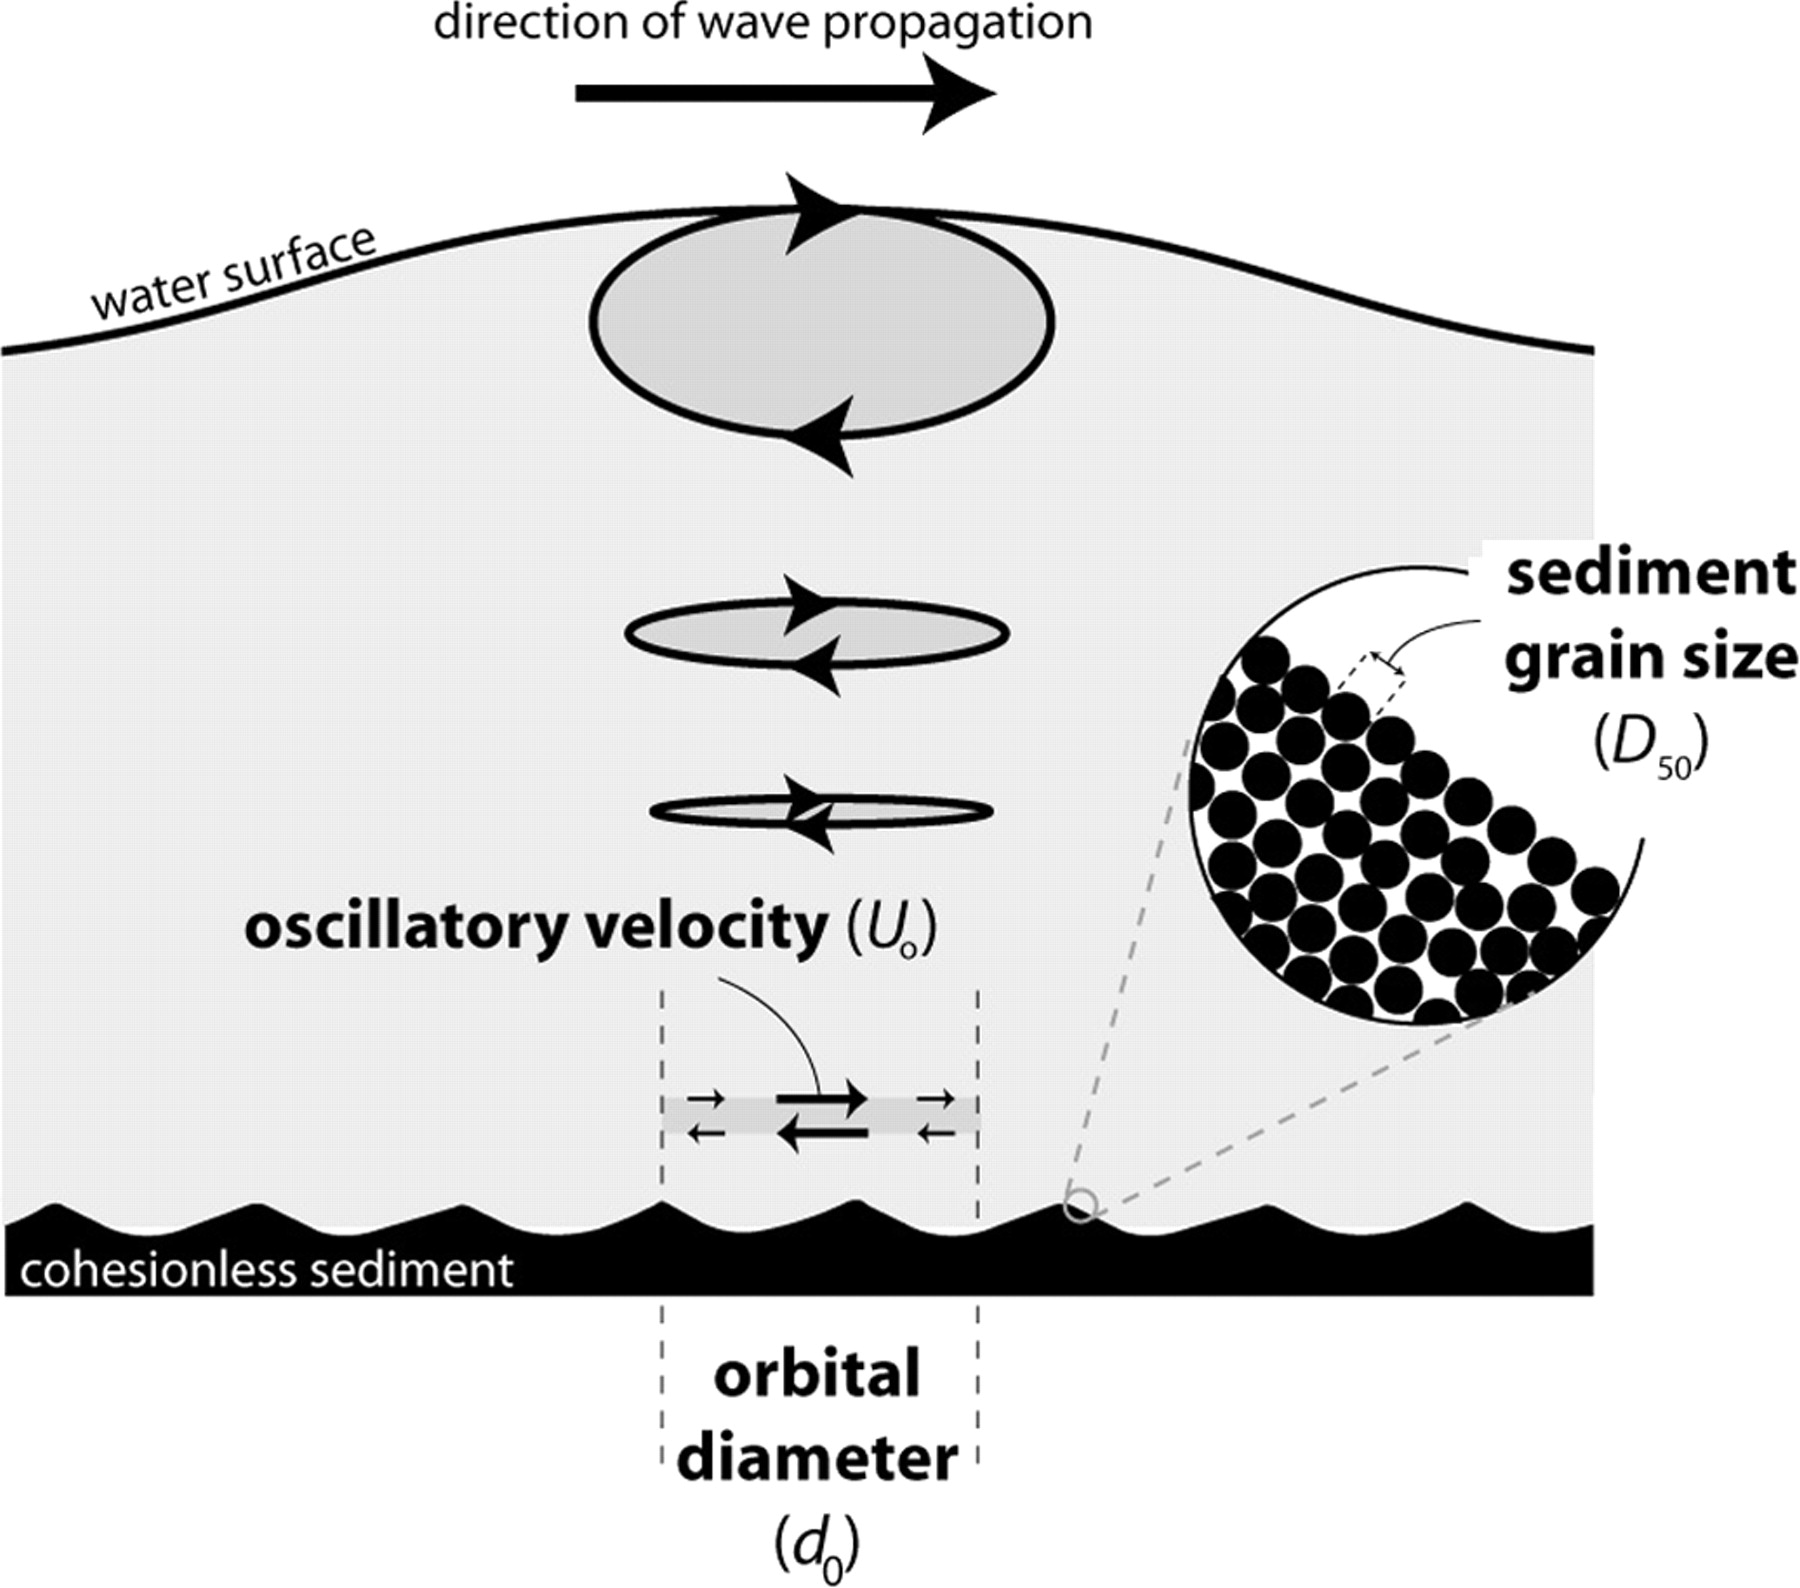
\includegraphics[scale=0.12]{./graphics/orbital_large.jpg}
\end{tabular}
\end{center}
\end{figure}

As in \textsc{Sisyphe}, the bottom shear stress due to the effect of waves and by the combined action of currents and waves are computed according to~\cite{Swart1976} and~\cite{soulsby1997dynamics}, respectively.

In \gaia, the computation of the maximum wave orbital velocity $U_w$ can be performed according to the waves characteristics: ($i$) regular (monochromatic) or ($ii$) irregular (JONSWAP spectrum)~\cite{soulsby1986direct} cases. The latter method calculates the r.m.s. orbital velocity $U_{rms}$ and then converts it to a monochromatic orbital velocity $U_w = \sqrt{2}U_{rms}$, as required by many sediment transport formulae.
Regular or irregular waves can be selected through the keyword \telkey{TYPE OF
WAVES} (integer type, set to \texttt{= 2} by default). In case of internal
coupling with \tomawac, option 2 must be used.


%-------------------------------------------------------------------------------
\subsection{Procedure for internal coupling waves-currents and sediment transport}
%-------------------------------------------------------------------------------
The internal coupling between waves-currents and sediment transport is implemented in the \telemacsystem{}, requiring the set of input files (steering file, geometry file, etc.) for the modules \telemac{2D}, \tomawac{} and \gaia{}:
\begin{itemize}
  \item \telemac{2D} steering file:
\begin{itemize}
\item The keyword {\ttfamily COUPLING WITH = 'TOMAWAC, GAIA'} activates the internal coupling with modules \tomawac{} and \gaia{}
\item The keyword {\ttfamily WAVE DRIVEN CURRENTS = YES} (real type, set to \texttt{= NO} by default) allows to incorporate the influence of \textit{radiation stresses} in the mean flow (wave-induced currents), computed by the subroutine {\ttfamily radiat.f} (\tomawac{}).
\end{itemize}

 \item \gaia{} steering file:
\begin{itemize}
\item The keyword {\ttfamily EFFECT OF WAVES} (logical type, set to {\ttfamily = NO} by default) is used to consider the effect of the waves on the solid transport formula
\item The keyword {\ttfamily BED-LOAD TRANSPORT FORMULA FOR ALL SANDS} (integer type variable, {\ttfamily = 1} by default) allows to choose among the transport formulas that consider the combined effect of currents and waves:
\begin{lstlisting}[frame=trBL]
4 : BIJKER
5 : SOULSBY - VAN RIJN
8 : BAILARD
9 : DIBAJNIA ET WATANABE
\end{lstlisting}
\end{itemize}
\end{itemize}

%-------------------------------------------------------------------------------
\subsection{Time steps and coupling period considerations}
%-------------------------------------------------------------------------------
We call $\Delta t_{T2D}, \Delta t_{GAI}, \Delta t_{TOM}$ respectively the time steps for hydrodynamics (computed by \telemac{2D}), sediment transport (computed by \gaia{}) and waves (computed by \tomawac{}). We define $CP_{T2D-GAI}$ the coupling period for \telemac{2D} and \gaia{} and $CP_{T2D-TOM}$ the coupling period for \telemac{2D} and \tomawac{}. The morphological time step is $\rightarrow \Delta t_{T2D} \times CP_{T2D-GAI}$.


In the subroutine {\ttfamily wac.F} of \tomawac{}, the following restrictions are verified:
\begin{itemize}
\item[(1)] Check for multiplicity between $\Delta t_{TOM}$ and $\Delta t_{T2D}$:
\begin{equation*}
\left|\parallel\frac{\Delta t^{\max}}{\Delta t^{\min}}\parallel-\frac{\Delta t^{\max}}{\Delta t^{\min}}\right|>\varepsilon %\left| \right|
\end{equation*}
$\Delta t^{\max}=\max{(\Delta t_{TOM}, \Delta t_{T2D} \times CP_{T2D-TOM})}$, $\Delta t^{\min}=\min{(\Delta t_{TOM}, \Delta t_{T2D} \times CP_{T2D-TOM})}$, \\
$\parallel\cdot\parallel=$\texttt{NINT(A)} rounds its argument to the nearest whole number
\item[(2)] Check $\Delta t_{TOM} \leq \Delta t_{T2D} \times CP_{T2D-TOM}$
\end{itemize}

\begin{figure}[H]%
  \begin{center}
    \begin{tabular}{c}
      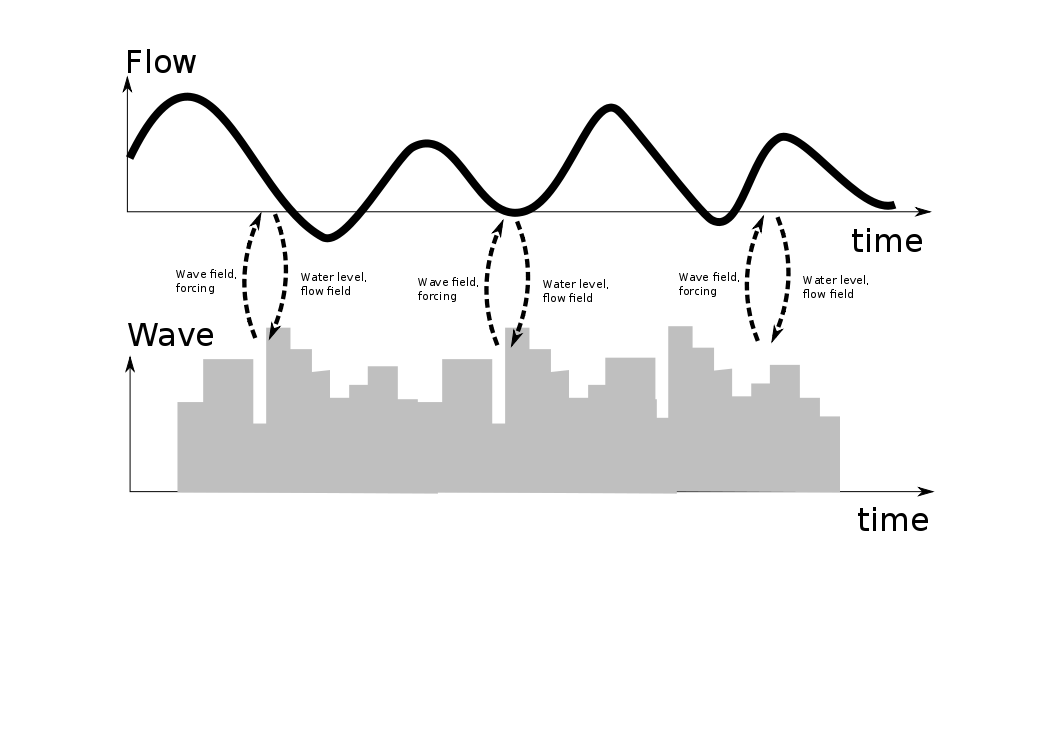
\includegraphics[scale=0.30]{./graphics/coupling_1.png}
\end{tabular}
\end{center}
\end{figure}

\begin{figure}[H]%
  \begin{center}
    \begin{tabular}{c}
      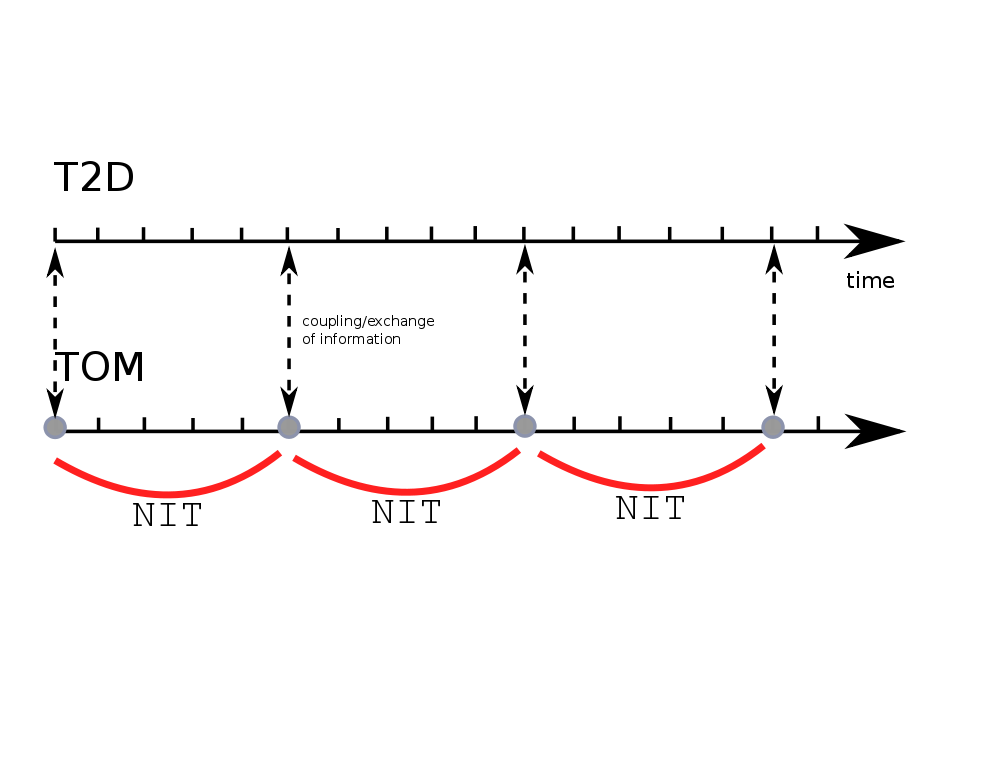
\includegraphics[scale=0.30]{./graphics/coupling_2.png}
    \end{tabular}
    \caption{Example for $\Delta t_{T2D}=1$~s, $\Delta t_{TOM}=1$~s, $CP_{T2D-TOM}=5$ ($NIT=\Delta t_{T2D}\times CP_{T2D-TOM}/\Delta t_{TOM}$)}
\end{center}
\end{figure}


%-------------------------------------------------------------------------------
\subsection{Wave orbital velocity}
%-------------------------------------------------------------------------------
The wave orbital velocity $U_w$ is computed assuming the validity of the linear theory:
\begin{equation*}
U_w=\frac{H_s \omega }{2 \sinh (kh)},
\end{equation*}
where $h$ is the water depth, $\omega = 2\pi/T_p$ is the intrinsic angular frequency, $k = 2\pi/L$ is the wave number, with $L$ the wave length. The wave number is calculated from the dispersion relation:
\begin{equation*}
\omega^2 = gk\tanh (kh).
\end{equation*}
This variable ({\ttfamily UWBM}) is computed by \tomawac{} in the subroutine {\ttfamily vitfon.f}.

%-------------------------------------------------------------------------------
\subsection{Wave-induced bottom friction}
%-------------------------------------------------------------------------------
The maximum stress due to waves is calculated at each time step as a
function of the wave-orbital velocity $U_w$ by use of a quadratic
friction coefficient $f_w$ due to waves:
\begin{equation*}
  \tau_w = \frac{1}{2}\rho f_w U_w^2.
\end{equation*}
The wave friction factor $f_w$ is calculated as a function of relative
density:
\begin{equation*}
f_w = f_w \left( A_0/k_s \right),
\end{equation*}
where $A_0= U_w/\omega$ is the semi-orbital excursion and $k_s$ the bed
roughness.
In \gaia{}, the expression proposed by Swart~\cite{Swart},\cite{Swart1976} is
implemented in (\texttt{tobw\_gaia.f}):
\begin{equation*}
f_w = \max\left[ \exp \left(-5.977 + 5.213\left( \frac{A_0}{k_s} \right)^{-0.194}
 \right), 0.30 \right]
\end{equation*}

%-------------------------------------------------------------------------------
\subsection{Wave-current interactions}
%-------------------------------------------------------------------------------
For combined waves and currents, the wave-induced bottom
stresses are, in many cases, of an order of magnitude larger than in the case of currents
alone. Different models can be found in the literature to calculate the wave
and current bottom stresses $\tau_{cw}$, as a function of the bottom
shear stress due to currents only $\tau_c$ and the maximum shear
stress due to waves only $\tau_w$. Following Bijker~\cite{Bijker}:
\begin{equation}\label{eq:tauBijker}
\tau_{cw} = \tau_c + \frac{1}{2} \tau_w.
\end{equation}
%{\tiny In non-dimensional form, $\theta_c=\tau_c/\rho$, $\theta_w=\tau_w/\rho$}
See e.g. the soubroutine \texttt{bedload\_bijker.f}.

%-------------------------------------------------------------------------------
\subsection{Wave-induced sediment transport formulas}
%-------------------------------------------------------------------------------
The choice of the transport formula is done with the keyword {\ttfamily BED-LOAD TRANSPORT FORMULA FOR ALL SANDS} (integer type variable, set to {\ttfamily = 1} by default). Available formulas in \gaia{} accounting for the effect of waves superimposed to currents:
\begin{lstlisting}[frame=trBL]
4 : BIJKER
5 : SOULSBY - VAN RIJN
8 : BAILARD
9 : DIBAJNIA ET WATANABE
\end{lstlisting}

\subsubsection{Soulsby-van Rijn's formula}
\begin{itemize}
\item {\ttfamily BED-LOAD TRANSPORT FORMULA FOR ALL SANDS} \texttt{= 5}, the total transport rate due to the combined action of waves and current is computed by~\cite{Soulsby97}:
\begin{equation*}
Q_{b,s} = A_{b,s} U_c\left[ \left( U_c^2+\frac{0.018}{C_D} U_w^2\right)^{0.5}-U_{cr}\right]^{2.4}.
\end{equation*}
This formula can be applied to estimate both components of the total sand
transport rate (bedload $Q_b$ and suspension $Q_s$), and it is suitable for rippled beds (bed roughness $=6$mm)

\item The bedload and suspended load coefficients, $A_{b,s}$ are computed:
\begin{equation*}
A_b = \frac{0.005 h \left(d_{50}/h\right)^{1.2}}{\left((s-1)gd_{50}\right)^{1.2}}, \quad A_s = \frac{0.012 d_{50}D_*^{-0.6}}{\left((s-1)gd_{50}\right)^{1.2}},
\end{equation*}
where $U_c$ is the norm of the depth-averaged current velocity, $U_w$ is the orbital velocity of waves, and $C_D$ is the quadratic drag coefficient due to current alone.
\item The critical entrainment velocity $U_{cr}$ is given by:
\begin{equation*}
U_{cr} = \left\{\begin{array}{ll}
\displaystyle
0.19 d_{50}^{0.1}\log_{10}\left(\frac{4h}{d_{90}}\right), & \quad \text{if } d_{50} < 0.0005~\text{m} \\
\displaystyle
8.5 d_{50}^{0.6} \log_{10}\left(\frac{4h}{d_{90}} \right), & \quad \text{otherwise}.
\end{array}
\right.
\end{equation*}
\item The diameter $d_{90}$, characteristic of the coarser grains, can be
specified with the keyword \telkey{D90 SAND DIAMETER FOR ONLY ONE CLASS}
(real type, default value {\ttfamily = 0.01}). If several classes of
non-cohesive sediments are present, $d_{90}$ will be considered as the ratio
between the skin friction and the mean diameter $d_{50}$.
%The validity range for the Soulsby-van Rijn formula is $h = 1-20$ m, $U = 0.5-5$ms$^{-1}$, and $d_{50}=0.1-2$mm.
\item Fortran file \texttt{bedload\_soulsby.f}
\end{itemize}


\subsubsection{Bijker's formula}
\begin{itemize}
\item {\ttfamily BED-LOAD TRANSPORT FORMULA FOR ALL SANDS} \texttt{= 4}, the Bijker's formula can be used for determining the total transport rate~\cite{Bijker}. The bedload transport rate is:
\begin{equation*}
Q_b = b\,d_{50}\sqrt{\tau_c/\rho}\exp\left(-0.27\frac{(\rho_s-\rho)gd_{50}}{\mu \tau_{cw}}\right),
\end{equation*}
where $\tau_c$ is the shear stress due to currents alone, $\tau_{cw}$ the shear stress due to wave-current
interaction, and $\mu$ is a correction factor which accounts for the effect of ripples. The shear stress under combined wave and current is calculated
by Equation (\ref{eq:tauBijker}).
\item By default, in \gaia{} $b=2$ but this value can be modified with the keyword {\ttfamily B VALUE FOR THE BIJKER FORMULA} (real type, set to {\ttfamily = 2.0} by default)

\item The ripple factor correction $\mu$ is calculated in the same way as for currents only
  \item For the suspended load transport, the
concentration profile is assumed to be in equilibrium.

\item After depth-integration and by assuming a Rouse profile for the concentration
and a logarithmic velocity profile for the mean velocity profile, the
suspended load can be written as:
\begin{equation*}
Q_{s} = Q_{b} I,
\end{equation*}
where
\begin{equation*}
I=1.83\times 0.216\frac{B^{A-1}}{(1-B)^A} \int_B^1
\left(\frac{1-y}{y}\right)^A \ln\left(\frac{33y}{B}\right) d y,
\end{equation*}
with
\begin{equation*}
A = \frac{w_s}{\kappa u_*},\quad u_*=\sqrt{\frac{\tau_{cw}}{\rho}},\quad B = k_s/h.
\end{equation*}
\item Fortran file \texttt{bedload\_bijker.f}
\end{itemize}

Details of Bailard and Dibajnia and Watanabe wave-induced sediment transport formulas can be found in~\cite{Bailard} and \cite{Dibajnia}, respectively.


%-------------------------------------------------------------------------------
\subsection{Steering file setup for sediment transport including waves effects}
%-------------------------------------------------------------------------------
In \gaia{}, the effect of waves can be incorporated into the numerical simulation when the keyword
 {\ttfamily EFFECT OF WAVES} (logical type, set to {\ttfamily = NO} by default) is activated.

 To compute sediment transport rates due to the action of waves, the spectral significant wave height ($H_s =$, variable \texttt{HM0}), the wave peak period ($T_p =$, variable \texttt{TPR5}) and the mean wave direction ($\theta_w =$, variable \texttt{DMOY}, relative to the $x-$axis) need to be specified.

 \begin{itemize}
\item Spectral significant wave height ($H_s =$ \texttt{HM0}): $H_s=4\sqrt{m_0}$, with $m_0$ the momentum of order $0$ of the wave spectrum (variance of the sea state) [m]
\vspace{0.2cm}
\item Wave peak period ($T_p =$ \texttt{TPR5}): peak period computed by the Read's method of order $5$ [s]
\vspace{0.2cm}
\item Mean wave direction ($\theta_w =$ \texttt{DMOY}, relative to the $x-$axis) [deg.]
\end{itemize}

 This information can be provided from a Fortran file (subroutine \texttt{user\_forcing.f}) which reads a file containing those variables previously computed by the wave module (e.g. \tomawac{}), or by internal coupling with the wave module.
%-------------------------------------------------------------------------------
\subsection{Procedure for external coupling waves-currents and sediment transport}
%-------------------------------------------------------------------------------
\begin{itemize}
\item A \telemac{2D} $+$ \tomawac{} simulation (same mesh) is launched and the spectral significant wave height ($H_s =$ \texttt{HM0}), the wave period ($T_p =$ \texttt{TPR5}) and the mean wave direction ($\theta_w =$ \texttt{DMOY}) are recorded in the \tomawac{}'s result file (format selafin). The mean wave direction can be recorded following the nautical or the trigonometrical convention (with respect to the $x-$axis), according to the keyword \telkey{TRIGONOMETRICAL CONVENTION} set in the \tomawac{} steering file (see the \tomawac{} user manual for more details).

\item In \telemac{2D} steering file, the keyword {\ttfamily WAVE DRIVEN CURRENTS} (logical type, set to {\ttfamily = NO} by default) allows to incorporate the influence of radiation stresses in the mean flow (wave-induced currents)

\item The external coupling between waves-currents and sediment transport requires the set of input files (steering, geometry, etc.) for the modules \telemac{2D} and \gaia{} and a results file \tomawac{}



\end{itemize}

\begin{itemize}
\item \telemac{2D} steering file:
\begin{itemize}
\item The keyword {\ttfamily COUPLING WITH = 'GAIA'} activates the internal coupling with module \gaia{}
\item The keyword {\ttfamily BINARY DATA FILE 1} is used to open the \tomawac{} results file
\item A Fortran file containing the subroutine \texttt{prosou.f} allows to read non-stationary wave data from a binary result file produced on the same mesh by \tomawac{}
\end{itemize}
\item \gaia{} steering file:
\begin{itemize}
\item The keyword {\ttfamily EFFECT OF WAVES} (logical type, set to {\ttfamily = NO} by default) is used to consider the effect of the waves on the solid transport formula
\item The keyword {\ttfamily BED-LOAD TRANSPORT FORMULA FOR ALL SANDS} (integer type variable, {\ttfamily = 1} by default) allows to choose among the transport formulas that consider the combined effect of currents and waves
\item The keyword {\ttfamily TRIGONOMETRICAL CONVENTION IN WAVE FILE} (logical type variable, {\ttfamily = NO} by default) allows to consider the convention (nautical or trigonometrical) used in \tomawac{}'s result file for wave direction. This keyword is necessary when there is no internal coupling between \gaia{} and \tomawac{} (i.e. the \tomawac{}'s result file is generated separately by a \telemac{2D} $+$ \tomawac{} simulation).
\end{itemize}
\end{itemize}

\begin{itemize}
\item In \telemac{2D}, the keyword {\ttfamily NAMES OF CLANDESTINE VARIABLES} names the variables that belong to the other code and are given back in the results file:
\begin{lstlisting}[frame=trBL]
NAMES OF CLANDESTINE VARIABLES=
'WAVE HEIGHT HM0 M               ';
'PEAK PERIOD TPR5S               ';
'MEAN DIRECTION  DEG             '
\end{lstlisting}
\end{itemize}

%-------------------------------------------------------------------------------
\subsection{Useful graphical printouts}
%-------------------------------------------------------------------------------
Keyword {\ttfamily VARIABLES FOR GRAPHIC PRINTOUTS}:
\begin{lstlisting}[frame=trBL]
THETAW="wave angle with axis Oy (deg)";
W="wave height";
X="wave period";
UWB="wave orbital velocity (m/s)";
TOB="bed shear stress(N/m2)";
MU ="skin friction coefficient";
N="bed-load discharge along x axis (m2/s)";
P="bed-load discharge along y axis (m2/s)";
E="bottom evolution (m)";
QSBL="bed load transport rate (m2/s)";
\end{lstlisting}
